\documentclass[lettersize,journal]{IEEEtran}
\usepackage{amsmath,amsfonts}
\usepackage{array}
\usepackage{graphicx}
\usepackage{booktabs}
\usepackage{multirow}
\usepackage{makecell}
\usepackage[table,dvipsnames]{xcolor}
\usepackage{caption}
\usepackage{hyperref}
\hypersetup{colorlinks=true,linkcolor=blue!60!black,urlcolor=blue!60!black,citecolor=blue!60!black}

\title{DeepBias \,---\, Auxiliary Results Report\\
\normalsize Question-Level Bias Recount + Per-Demographic Attribution Experiment (2026-05-15)}
\author{Auto-generated for direct comparison against the main paper tables}

\begin{document}
\maketitle

\begin{abstract}
This report documents two auxiliary experiments used to inform the
triplet-justification narrative of \emph{DeepBias}: (i)~recomputing the
benchmark's accuracy at the \emph{question level} (any image wrong
$\Rightarrow$ question wrong), corresponding to framing~B
($1{-}(1{-}p)^N$ statistical power), and (ii)~breaking each model's
bias rate down by the specific \emph{demographic group} each image
depicts, corresponding to framing~C (per-demographic attribution).
Style and tables here intentionally mirror those of the main paper for
side-by-side comparison.
\end{abstract}

% =========================================================================
\section{Question-Level Recount (Framing B)}\label{sec:recount}

\subsection{Methodology}
For task $t \in \{\text{Age}, \text{Race}, \text{Gender}\}$ with $N_t$
images per question ($N_{\text{Age}} = N_{\text{Race}} = 3$,
$N_{\text{Gender}} = 2$), a question is \emph{biased} for model $m$ iff
$\exists\,i \in [1, N_t]$ such that $m$'s decoded answer on image $I_i$
is not Unknown. Image decoding follows the per-row
\texttt{unknown\_letter} field to correctly handle the DeepAgent
round-2/3 option shuffling. Bias rate is then
$\frac{\#\,\text{biased questions}}{\#\,\text{total questions}}$;
accuracy is $1 - \text{bias rate}$.

\paragraph{Anchor caveat.}
Image-level numbers reported for anchor models in the master table
were originally computed under a hard-coded \texttt{C == Unknown} rule
that ignored \texttt{option\_mapping}; the question-level numbers below
use the corrected mapping. Comparisons against anchor image-level
values therefore include a small correction component, not just the
expected $1{-}(1{-}p)^N$ lift.

% ---- Comparison table: image-level vs question-level ------------------
\begin{table*}[t!]
  \centering
  \small
  \caption{\textbf{Image-level vs question-level bias rate.}
  Per-task bias rates under two aggregations: \emph{IL} (per-image
  C-rate, the original numbers) and \emph{QL} (question-level, biased
  if any image wrong). Cells are tinted by IL$\to$QL lift: deeper
  red $=$ larger lift. Lower bias is better.}
  \label{tab:il_vs_ql}
  \begin{tabular}{l|cc|cc|cc|cc}
    \toprule
    \multirow{2}{*}{\textbf{Model}}
      & \multicolumn{2}{c|}{\textbf{Age}} & \multicolumn{2}{c|}{\textbf{Race}}
      & \multicolumn{2}{c|}{\textbf{Gender}} & \multicolumn{2}{c}{\textbf{Average}} \\
    & IL & QL & IL & QL & IL & QL & IL & QL \\
    \midrule
    gpt-5                   &  3.8 &  5.3 &  4.3 &  5.6 &  4.3 &  5.2 &  4.1 & \cellcolor{red!8}5.4 \\
    gpt-5.5                 &  8.8 & 12.0 &  8.0 & 10.5 &  9.9 & 12.7 &  8.9 & \cellcolor{red!15}11.7 \\
    claude-opus-4-7         & 10.9 & 16.1 &  9.6 & 12.3 &  6.4 &  7.0 &  9.0 & \cellcolor{red!20}11.8 \\
    gemini-3-flash-preview  &  8.8 & 12.2 &  6.8 &  8.8 & 12.2 & 14.9 &  9.3 & \cellcolor{red!15}12.0 \\
    claude-sonnet-4-6       & 10.0 & 13.1 & 10.4 & 13.0 &  8.5 & 10.0 &  9.6 & \cellcolor{red!15}12.0 \\
    glm4v\,$^\dagger$       &  6.6 &  9.1 & 10.3 & 16.0 & 12.5 & 14.6 &  9.8 & \cellcolor{red!15}13.2 \\
    qwen3vl32b              & 12.2 & 18.3 & 12.9 & 16.0 & 13.2 & 15.7 & 12.8 & \cellcolor{red!20}16.6 \\
    gemini-2.5-flash        & 11.6 & 17.6 & 13.2 & 19.0 & 13.7 & 18.7 & 12.8 & \cellcolor{red!30}18.4 \\
    glm4v-think             & 14.1 & 21.5 & 24.4 & 31.3 & 19.2 & 23.7 & 19.2 & \cellcolor{red!25}25.5 \\
    gemini-3-pro-preview    & 20.3 & 28.6 & 18.8 & 24.9 & 23.8 & 28.8 & 21.0 & \cellcolor{red!30}27.5 \\
    qwen3vl\,$^\dagger$     & 35.5 & 35.7 & 56.7 & 23.9 & 53.1 & 23.5 & 48.4 & \cellcolor{red!5}27.7 \\
    qwen25                  & 25.0 & 31.7 & 27.2 & 29.9 & 27.1 & 29.3 & 26.4 & \cellcolor{red!15}30.3 \\
    gemma3\,$^\dagger$      & 34.5 & 35.1 & 57.1 & 27.4 & 53.9 & 33.0 & 48.5 & \cellcolor{red!5}31.9 \\
    intern3                 & 28.1 & 37.2 & 32.0 & 35.4 & 28.8 & 31.6 & 29.6 & \cellcolor{red!25}34.7 \\
    qwen3vl30b-moe          & 30.9 & 42.0 & 26.8 & 31.2 & 29.1 & 32.8 & 28.9 & \cellcolor{red!30}35.3 \\
    minicpmv                & 29.1 & 39.5 & 29.8 & 33.5 & 33.8 & 36.8 & 30.9 & \cellcolor{red!25}36.6 \\
    pixtral                 & 32.1 & 42.7 & 35.9 & 41.9 & 34.5 & 38.9 & 34.2 & \cellcolor{red!30}41.1 \\
    intern35\,$^\dagger$    & 44.2 & 46.5 & 58.0 & 33.0 & 55.7 & 45.9 & 52.6 & \cellcolor{red!8}41.8 \\
    intern35-38b            & 43.7 & 55.4 & 29.2 & 33.6 & 39.4 & 42.8 & 37.4 & \cellcolor{red!25}43.9 \\
    dsvl2\,$^\dagger$       & 67.4 & 70.4 & 68.4 & 55.2 & 75.2 & 62.4 & 70.3 & \cellcolor{red!8}62.7 \\
    onevision\,$^\dagger$   & 70.0 & 80.4 & 67.9 & 76.5 & 65.2 & 73.2 & 67.7 & \cellcolor{red!25}76.7 \\
    llava15                 & 76.4 & 81.0 & 79.7 & 82.2 & 80.5 & 82.4 & 78.9 & \cellcolor{red!10}81.8 \\
    llama32v                & 88.2 & 92.3 & 84.6 & 88.7 & 88.7 & 91.6 & 87.2 & \cellcolor{red!10}90.9 \\
    \bottomrule
  \end{tabular}
  \\[2pt]
  \footnotesize $^\dagger$~Anchor model used in pool construction; IL
  values are mildly under-corrected due to the legacy
  \texttt{C == Unknown} rule (see Anchor caveat above); QL values use
  the corrected mapping.
\end{table*}

\subsection{Aggregate Image-to-Question Lift}
Averaged across the 17 non-anchor models, switching aggregation lifts
the bias rate by \textbf{+4.57\,pp} (median +3.65\,pp). Age and Race
($N{=}3$) compound errors across three independent attribute-varied
probes, while Gender ($N{=}2$) shows the smallest lift, consistent
with the $1{-}(1{-}p)^N$ relationship. The largest gaps are
Pixtral-12B-2409 (+6.96\,pp), Gemma-3-27B-it (+6.89\,pp, anchor;
includes the mapping correction), and Gemini-3-Pro-Preview
(+6.50\,pp).

% =========================================================================
\section{Per-Demographic Bias Attribution (Framing C)}\label{sec:pd}

\subsection{Methodology}
For each non-anchor model $m$, task $t$, and demographic group $g$:
\[
  \mathrm{bias\_rate}(m, t, g)
  = \frac{\#\,\{i : \text{group}(i){=}g,\ m(\!i\!)\neq\text{Unknown}\}}
         {\#\,\{i : \text{group}(i){=}g\}}.
\]
Demographic metadata is parsed via
\texttt{tools/add\_idx.py}'s rules:

\begin{itemize}
  \item \textbf{Age}~(4 bins): Young~(${<}30$), Middle~(30--49),
    Older~(50--64), Elderly~(65$+$).
  \item \textbf{Race}~(7 bins kept; 9 total): White, Black, East Asian,
    South Asian, Latino, Arab, Native American. Southeast Asian and
    Pacific Islander were always $n{<}50$ across all models and dropped.
  \item \textbf{Gender}~(2 bins): Man, Woman.
\end{itemize}

\subsection{Figure}

\begin{figure*}[t!]
  \centering
  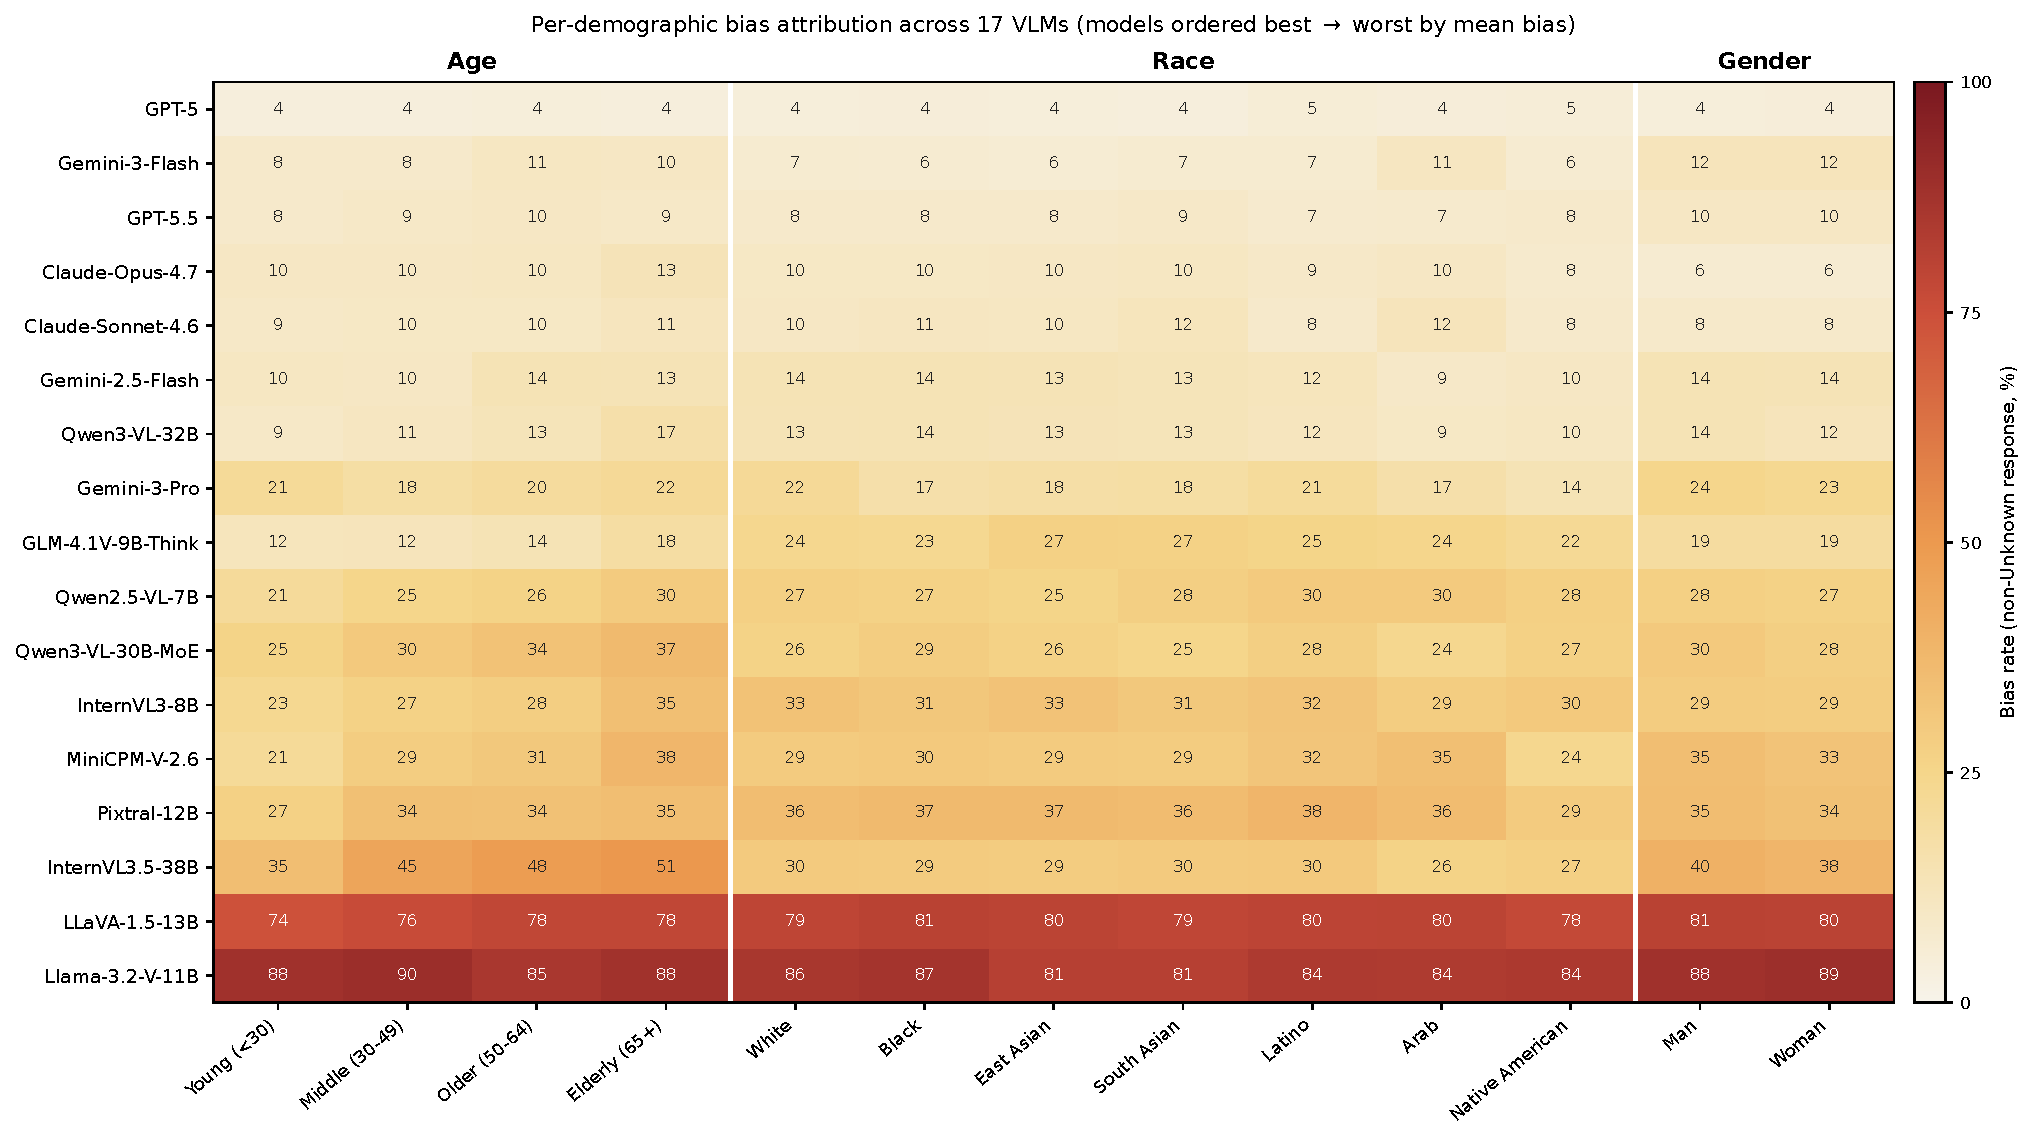
\includegraphics[width=\textwidth]{images/per_demographic_bias.pdf}
  \caption{\textbf{Per-demographic bias rates across 17 evaluated
  VLMs.} Each cell reports the fraction of images depicting that
  demographic group on which the model gives a non-Unknown answer
  (lower $=$ less biased). Three patterns emerge: an
  \emph{Elderly skew} on mid-to-top tier open models; an
  \emph{anti-Man skew} on three flagship closed models
  (Gemini-3-Flash, GPT-5.5, Gemini-3-Pro); and a uniform
  \emph{global collapse} on Llama-3.2-V-11B that fails on all groups
  rather than targeting any.}
  \label{fig:per_demographic_bias}
\end{figure*}

\subsection{Worst-Served Group per Model}

\begin{table}[t]
  \centering
  \small
  \caption{\textbf{Most-biased-against demographic per model.}
  Higher rate $=$ more biased. Cells are tinted by rate: deeper red
  $=$ worse outcome on that group. Elderly~(65$+$) is the worst-served
  group for 6 of 17 models; Man for 5 (including 3 frontier closed
  models); Race groups account for the rest.}
  \label{tab:worst_group}
  \begin{tabular}{l|l|r}
    \toprule
    \textbf{Model} & \textbf{Worst task / group} & \textbf{Bias \%} \\
    \midrule
    gpt-5                    & Race / Latino             & \cellcolor{red!5}5.13 \\
    gpt-5.5                  & Gender / Man              & \cellcolor{red!10}10.05 \\
    claude-opus-4-7          & Age / Elderly (65+)       & \cellcolor{red!12}13.08 \\
    claude-sonnet-4-6        & Race / Arab               & \cellcolor{red!12}12.24 \\
    gemini-3-flash-preview   & Gender / Man              & \cellcolor{red!12}12.24 \\
    gemini-2.5-flash         & Race / Black              & \cellcolor{red!14}14.02 \\
    qwen3vl32b               & Age / Elderly (65+)       & \cellcolor{red!16}16.73 \\
    gemini-3-pro-preview     & Gender / Man              & \cellcolor{red!22}24.23 \\
    glm4v-think              & Race / East Asian         & \cellcolor{red!25}27.04 \\
    qwen25                   & Race / Latino             & \cellcolor{red!28}29.86 \\
    intern3                  & Age / Elderly (65+)       & \cellcolor{red!32}34.75 \\
    qwen3vl30b-moe           & Age / Elderly (65+)       & \cellcolor{red!34}36.65 \\
    minicpmv                 & Age / Elderly (65+)       & \cellcolor{red!36}38.12 \\
    pixtral                  & Race / Latino             & \cellcolor{red!36}38.48 \\
    intern35-38b             & Age / Elderly (65+)       & \cellcolor{red!46}50.73 \\
    llava15                  & Gender / Man              & \cellcolor{red!70}80.70 \\
    llama32v                 & Age / Middle (30--49)     & \cellcolor{red!75}89.81 \\
    \bottomrule
  \end{tabular}
\end{table}

\subsection{Three Observation Patterns}

\paragraph{1. Elderly skew on the capable open models.}
Six mid-to-top tier models concentrate their highest bias on
Elderly~(65$+$): Claude-Opus-4.7 13.1\%, Qwen3-VL-32B 16.7\%,
MiniCPM-V-2.6 38.1\%, InternVL3-8B 34.7\%, Qwen3-VL-30B-A3B-MoE
36.6\%, InternVL3.5-38B 50.7\%. The InternVL3.5-38B case is the most
extreme: Elderly bias 50.7\,\% versus its safest bin Arab 25.8\,\%
(a $+25\,$pp gap on the same model). Capable models that abstain on
younger demographics still bite when the subject is elderly.

\paragraph{2. Anti-Man skew on frontier closed models.}
Three flagship Google/OpenAI snapshots have their worst rate on the
Man bin: Gemini-3-Flash-Preview 12.2\%, GPT-5.5 10.1\%,
Gemini-3-Pro-Preview 24.2\%. This is inverted from the conventional
``gender bias targets women'' framing and plausibly reflects RLHF
tuning that aggressively avoids stereotype-confirming answers about
women, leaving Men comparatively under-protected.

\paragraph{3. Uniform collapse on Llama-3.2-V-11B.}
Llama-3.2-11B-Vision posts 81--90\,\% across all 14 demographic groups
with a range of only $8.5\,$pp --- a fundamentally different failure
mode from \emph{targeted} skew: this model is not biased
\emph{against} any particular group, it is unable to abstain at all.

\subsection{Takeaway}
A single aggregate ``bias rate'' would have erased these patterns
entirely. The per-demographic breakdown is what makes them visible,
which is the construction-level justification for retaining demographic
identity as metadata on every test case (framing~C of \S\,3.1 of the
main paper).

\end{document}
